\documentclass[12pt,a4paper,oneside]{book}

\usepackage{graphicx}

\usepackage{enumitem}
\usepackage{amsmath}


\begin{document}

\tableofcontents

\chapter{Introduction}


\chapter{This is my first chapter}\label{ch:1}

This is some normal text.

{\Huge
	This is little bigger
}

\begin{center}
This will be aligned center.
\end{center}


\begin{flushright}
	This is right aligned.
\end{flushright}

\begin{flushleft}
Lorem Ipsum is simply dummy text of the printing and typesetting industry. Lorem Ipsum has been the industry's standard dummy text ever since the 1500s, when an unknown printer took a galley of type and scrambled it to make a type specimen book. It has survived not only five centuries, but also the leap into electronic typesetting, remaining essentially unchanged. It was popularised in the 1960s with the release of Letraset sheets containing Lorem Ipsum passages, and more recently with desktop publishing software like Aldus PageMaker including versions of Lorem Ipsum.
\end{flushleft}


Lorem Ipsum is simply dummy text of the printing and typesetting industry. Lorem Ipsum has been the industry's standard dummy text ever since the 1500s, when an unknown printer took a galley of type and scrambled it to make a type specimen book. It has survived not only five centuries, but also the leap into electronic typesetting, remaining essentially unchanged. It was popularised in the 1960s with the release of Letraset sheets containing Lorem Ipsum passages, and more recently with desktop publishing software like Aldus PageMaker including versions of Lorem Ipsum.

Something



\section{How to insert Figures}

jjdhf;jd;lk
dfjdkfj;d
dfjdjlkf


\begin{figure}[htb!]
	\centering
	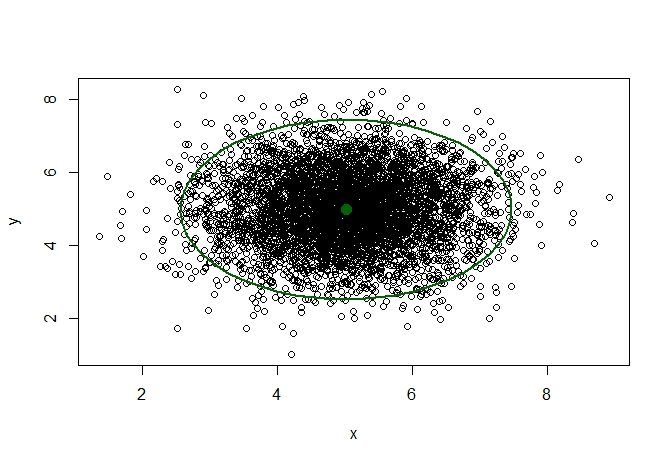
\includegraphics[scale=.5]{images/Rplot}
	\caption{Confidence Ellipses}
\end{figure}


jfdkj
4

\begin{figure}[htb!]
	\centering
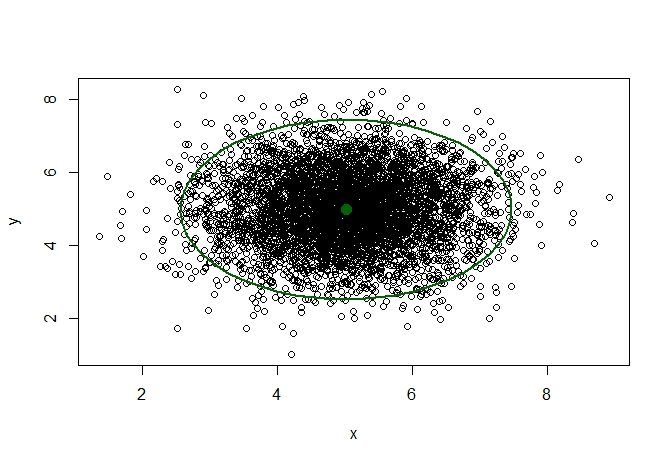
\includegraphics[scale=.5]{images/Rplot}
\caption{Confidence Ellipses}
\label{fig:conf_ellipse}
\end{figure}


In Figure \ref{fig:conf_ellipse}, we have plotted the confidence ellipses. 

\clearpage 
\section{How to type enumerations}

\begin{enumerate}[label = {[O\arabic*]}]
	\item\label{it:1}This is the first item 
	
	\item This is the second item 
\end{enumerate}

In Item \ref{it:1} we discuss something. ..


\section{How to type aligned equations}


\begin{equation}\label{eq:1}
 f(x) = x^2
\end{equation}


The equation \ref{eq:1} tells about....




\begin{align}
	f(x) & = x^2\nonumber \\
	    & = x\times x
\end{align}



\begin{align*}
f(x) & = x^2\\
& = x\times x
\end{align*}

\textbf{This is bold}

\textbf{\large This is little bigger bold font}

\textit{This is italics.... }



\chapter{This is my second chapter}


In Chapter \ref{ch:1}, we discussed how to insert figures. 


\end{document}